\chapter{Lattice dynamics in LSCO+O: A study using ToF and ab-initio MD}\label{ch:in4}

\begin{framed}
    \begin{itemize}
        \item Presentation of data
        \item Comparison with simulations
        \item LTT/LTO discussion. 
        \item What does the phrase `LTT-like tilts' actually mean. Is it important?
    \end{itemize}
\end{framed}


\section{Introduction}
We are performing inelastic neutron time-of-flight experiments on a series of La$_{2-x}$Sr$_{x}$CuO$_{4+\delta}$ powdered samples in order to better understand the curious relationship between mobile (O) and static (Sr) dopants. By careful analysis of the changes in the phonon spectra, we hope to better understand the role of mobile dopants and their relationship to superconductivity.

\section{Samples}
Experiments were performed on 4 powdered samples of roughly 5 grams each: LCO (no $T_\text{c}$), LSCO (no $T_\text{c}$), LCO+O ($T_\text{c} = \SI{40}{\kelvin}$), LSCO3+O ($T_\text{c} = \SI{40}{\kelvin}$). Powders were synthesized by mixing \ce{La2O3}, \ce{CuO} and (in the case of Sr doping) \ce{SrCO3} followed by calcination in a box furnace at 950$^\circ \, \text{C}$ for 48 hours. Intercalation of oxygen was performed by electrochemical methods at University of Copenhagen. This method has previously been described elsewhere \cite{Blakeslee1998}.

\section{Experimental}
Experiments were performed at the thermal neutron time-of-flight spectrometer IN4c at Institut Laue-Langevin in Grenoble, France. In order to see excitations in the \SIrange{5}{100}{\milli\eV} range, each sample/temperature was measured at three different incident neutron wavelengths as shown in Table \ref{tab:in4_mono}. Sample was mounted in a cadmium frame as shown in Figure \ref{fig:sample_sqw}B. Each of the 4 samples was measured for 3.5-4 hours per temperature/wavelength combination. 

\begin{figure}
    \centering
    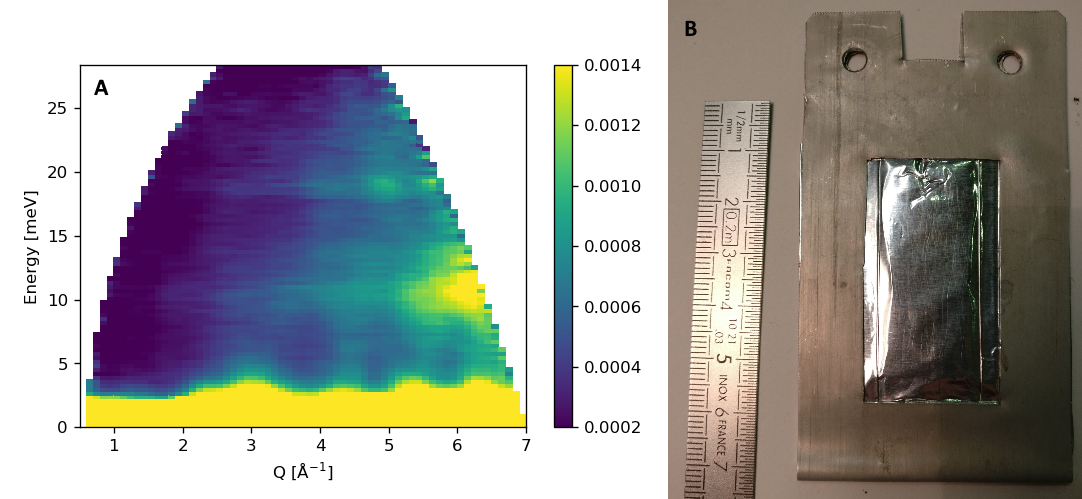
\includegraphics[width=\textwidth]{fig/gdos/sample_sqw.png}
    \caption[$S(\bm{q}, \omega)$ map and picture of sample]{\textbf{A}: $S(\bm{q}, \omega)$ map of LSCO at \SI{10}{K} with $\lambda = \SI{1.6}{\angstrom}$ incident wavelength. Data has normalized by the Bose factor. \textbf{B:} Sample mounted in cadmium frame.}
    \label{fig:sample_sqw}
\end{figure}

\begin{table}[b]
    \centering
    \begin{tabular}{lllll}\toprule
    $\lambda$ [\AA] & Monochromator  & $k$ [\AA$^{-1}$] & E [meV] & Sapphire Filter     \\ \midrule
    1.6             & PG004 & 3.93            & 31.95   & \texttt{IN}  \\
    1.1             & PG004 & 5.71            & 67.61   & \texttt{IN}  \\
    0.85            & Cu220 & 7.39            & 113.22  & \texttt{OUT} \\ \bottomrule
    \end{tabular}
    \caption[IN4: Incident energies]{Overview of incident energies used in the experiments.}
    \label{tab:in4_mono}
\end{table}

The raw time-of-flight data was reduced to $S(\bm{q},\omega)$ using the \texttt{Mantid} \cite{Arnold2014} software. Background was corrected using a Vanadium scan. Due to the isotropic nature of the powder, we only consider the magnitude of $\bm{q}$ and the resulting data can be viewed in two dimensions as shown in Figure \ref{fig:sample_sqw}A. Obtaining the density-of-states is done in Mantid with the \texttt{ComputeIncoherentDOS} algorithm, using the following expression for the 1-phonon incoherent scattering function:

 \[ S^{(1)}_{\mathrm{inc}}(Q,E) = \exp\left(-2\bar{W}(Q)\right) \frac{Q^2}{E} \langle n+\frac{1}{2}\pm\frac{1}{2} \rangle \left[ \sum_k \frac{\sigma_k^{\mathrm{scatt}}}{2m_k} g_k(E) \right]\, , \]
 
 \noindent where $\bar{W} = Q^2 \langle u^2 \rangle / 2$ with $\langle u^2 \rangle$ being the average mean-squared displacement. $n$ is the Bose factor and $E$ is the energy transfer. Finally, the term in brackets is the neutron-weighted density of states with $k$ running over the different elements in our sample. The calculated DOS is given in milibarns/steredians per formula unit per meV. The mean squared displacement was set to $\langle u^2 \rangle = \SI{0.015}{\angstrom}$, which is a good compromise between qualitatively describing our data and the actual values of $\langle u^2 \rangle$ as obtained from experiments \todo{cite hafliger} and simulations \todo{cite and create MSD figure}.
 
 In order to get meaningful results from this procedure, reduction of the raw data is usually required. Generally, one chooses a range of $Q$ and $E$ to sum over along with a re-binning of $E$. Since the measured ranges are different between incident energies, these ranges are chosen for each of the three configurations (see Table \ref{tab:in4_mono}). The parameters used for our calculations are shown in Table \ref{tab:qeranges}.
 
\begin{table}[b]
   \centering
   \begin{tabular}{llllll}
   \toprule
   $\lambda$ [\AA] & $Q_\text{min}$ [\AA$^{-1}$] & $Q_\text{max}$ [\AA$^{-1}$] & $E_\text{min}$ [meV] & $E_\text{max}$ [meV] & $\Delta E$ [meV] \\ \midrule
   1.6             & 2.0                         & 7.0                         & 4.0                  & 26.0                 & 0.2              \\
   1.1             & 3.0                         & 10.0                        & 7.0                  & 59.0                 & 0.4              \\
   0.85            & 4.0                         & 12.0                        & 15.0                 & 98.0                 & 1.0              \\ \bottomrule
   \end{tabular}
    \caption[IN4: $Q$ and $E$ windows for DOS integration]{$Q$ and $E$-ranges used in the computation of DOS. For all specta a mean squared displacement of $\langle u^2 \rangle = \SI{0.015}{\angstrom}$ was used.}
    \label{tab:qeranges}
\end{table}

\section{Results}
In order to visualize our spectra better, we start by stiching the different wavelengths together. Since the energy resolution of the instrument worsens with increasing incomming energy $E_i$ we stitch together data from the different wavelengths, such that the $\lambda = \SI{1.6}{\angstrom}$ data describes low energies up to $\approx \SI{24}{\milli\electronvolt}$, $\lambda = \SI{1.1}{\angstrom}$ data describes intermediate energies up to $\approx \SI{43}{\milli\electronvolt}$ and $\lambda = \SI{0.85}{\angstrom}$ data descibes high energy data.

Data is stitched together by chosing some cut-off energies such that no features are introduced when we combine the data. The data for $\lambda = \SI{1.1}{\angstrom}$ and $\lambda = \SI{0.85}{\angstrom}$ is then scaled such that we get a continuous spectrum across the full range. For this reason, the absolute values of the DOS is only representative for the $\lambda = \SI{1.6}{\angstrom}$ data. Figure \ref{fig:in4_stitch} shows the result of such a concatenation of data. In addition, vertical lines have been added to show qualitative features of the spectrum.

\begin{figure}
    \centering
    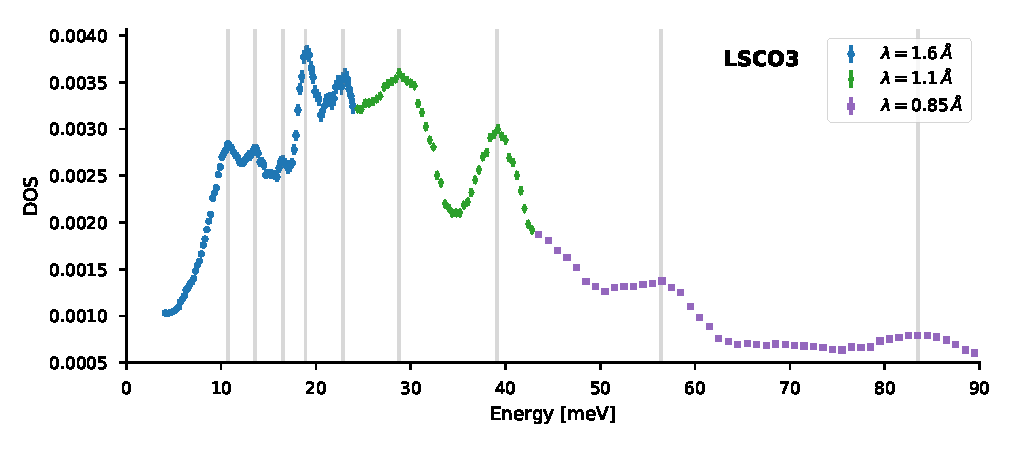
\includegraphics[width=\textwidth]{fig/gdos/in4_lsco3_10k.pdf}
    \caption[gDOS of LSCO3 at 10K. Visualize stitching of data.]{DOS of the LSCO3 }
    \label{fig:in4_stitch}
\end{figure}


\begin{figure}
    \centering
    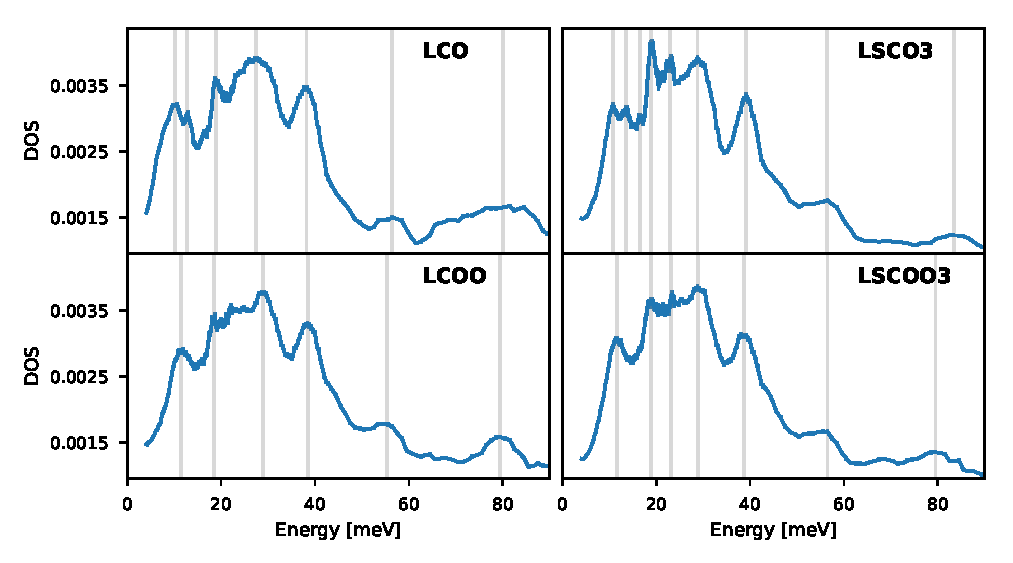
\includegraphics[width=\textwidth]{fig/gdos/in4_10K.pdf}
    \caption[gDOS at \SI{10}{\kelvin}]{GDOS at \SI{10}{\kelvin}}
    \label{fig:gdos_10k}
\end{figure}

\begin{figure}
    \centering
    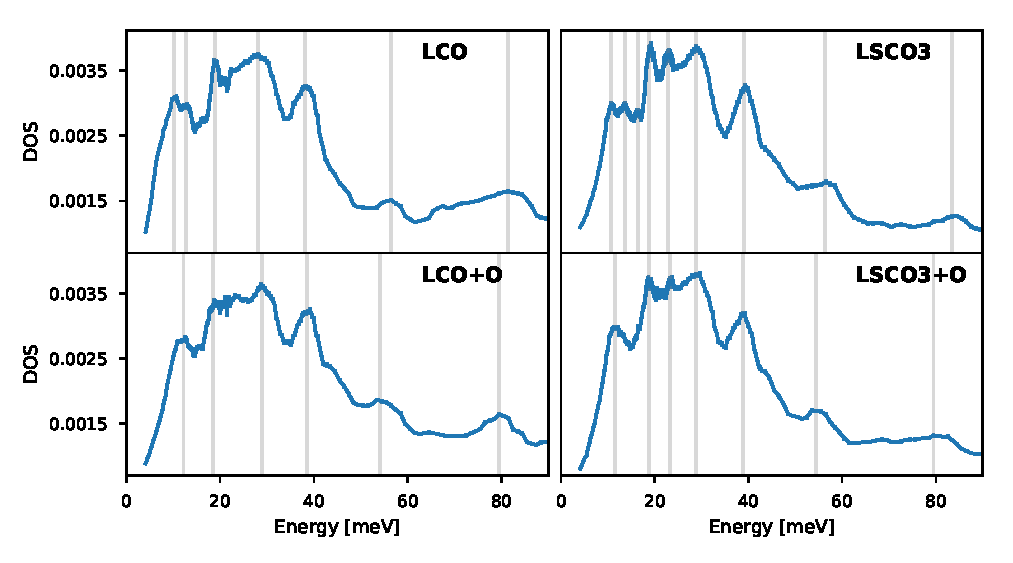
\includegraphics[width=\textwidth]{fig/gdos/in4_60K.pdf}
    \caption[gDOS at \SI{60}{\kelvin}]{GDOS at \SI{60}{\kelvin}}
    \label{fig:gdos_60k}
\end{figure}

\begin{figure}
    \centering
    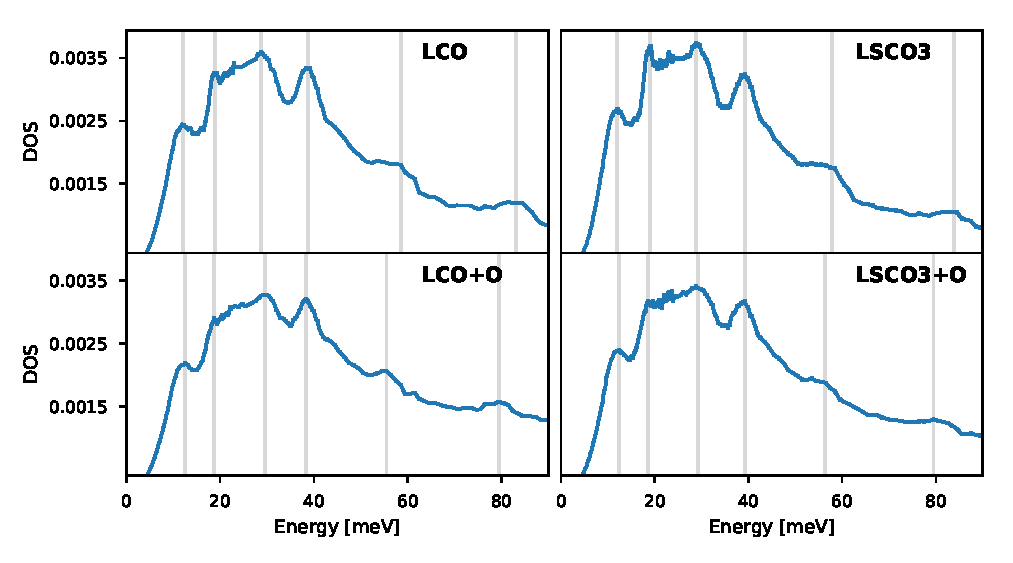
\includegraphics[width=\textwidth]{fig/gdos/in4_300K.pdf}
    \caption[gDOS at \SI{300}{\kelvin}]{GDOS at \SI{300}{\kelvin}}
    \label{fig:gdos_300k}
\end{figure}

\begin{figure}[]
    \centering
    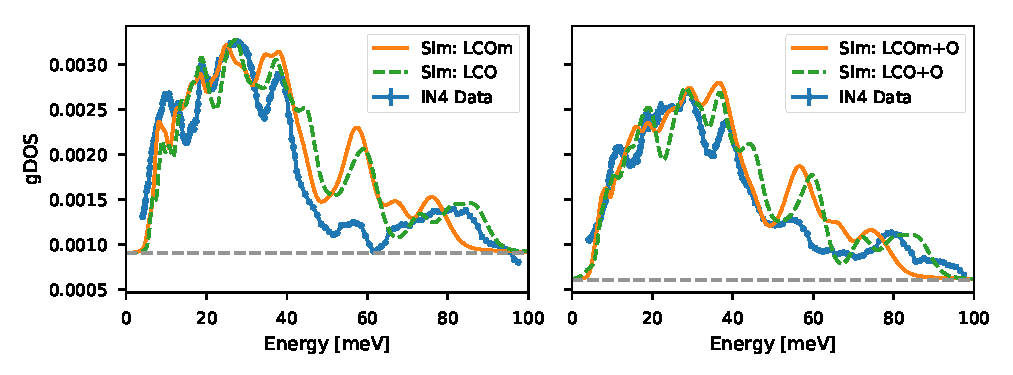
\includegraphics[width=\textwidth]{fig/gdos/gdos_simulation_experiment_compare.pdf}
    \caption[compare gdos simulation]{compare gdos simulation. Seems like metallic simulations are not that important for structure, but the dynamics become modified in a meaningful way!. The simulation data is smoothed by a gaussian width that depends on the energy $\sigma = 0.4 + 0.02 E$ [meV].}
    \label{fig:compare_gdos_sim}
\end{figure}